\section{Day 23: Functors; Retracts, Brouwer Fixed Point (Nov. 26, 2024)}
Outfit of the day: monocolor sweater. that's a second
\begin{figure}[h]
    \centering
    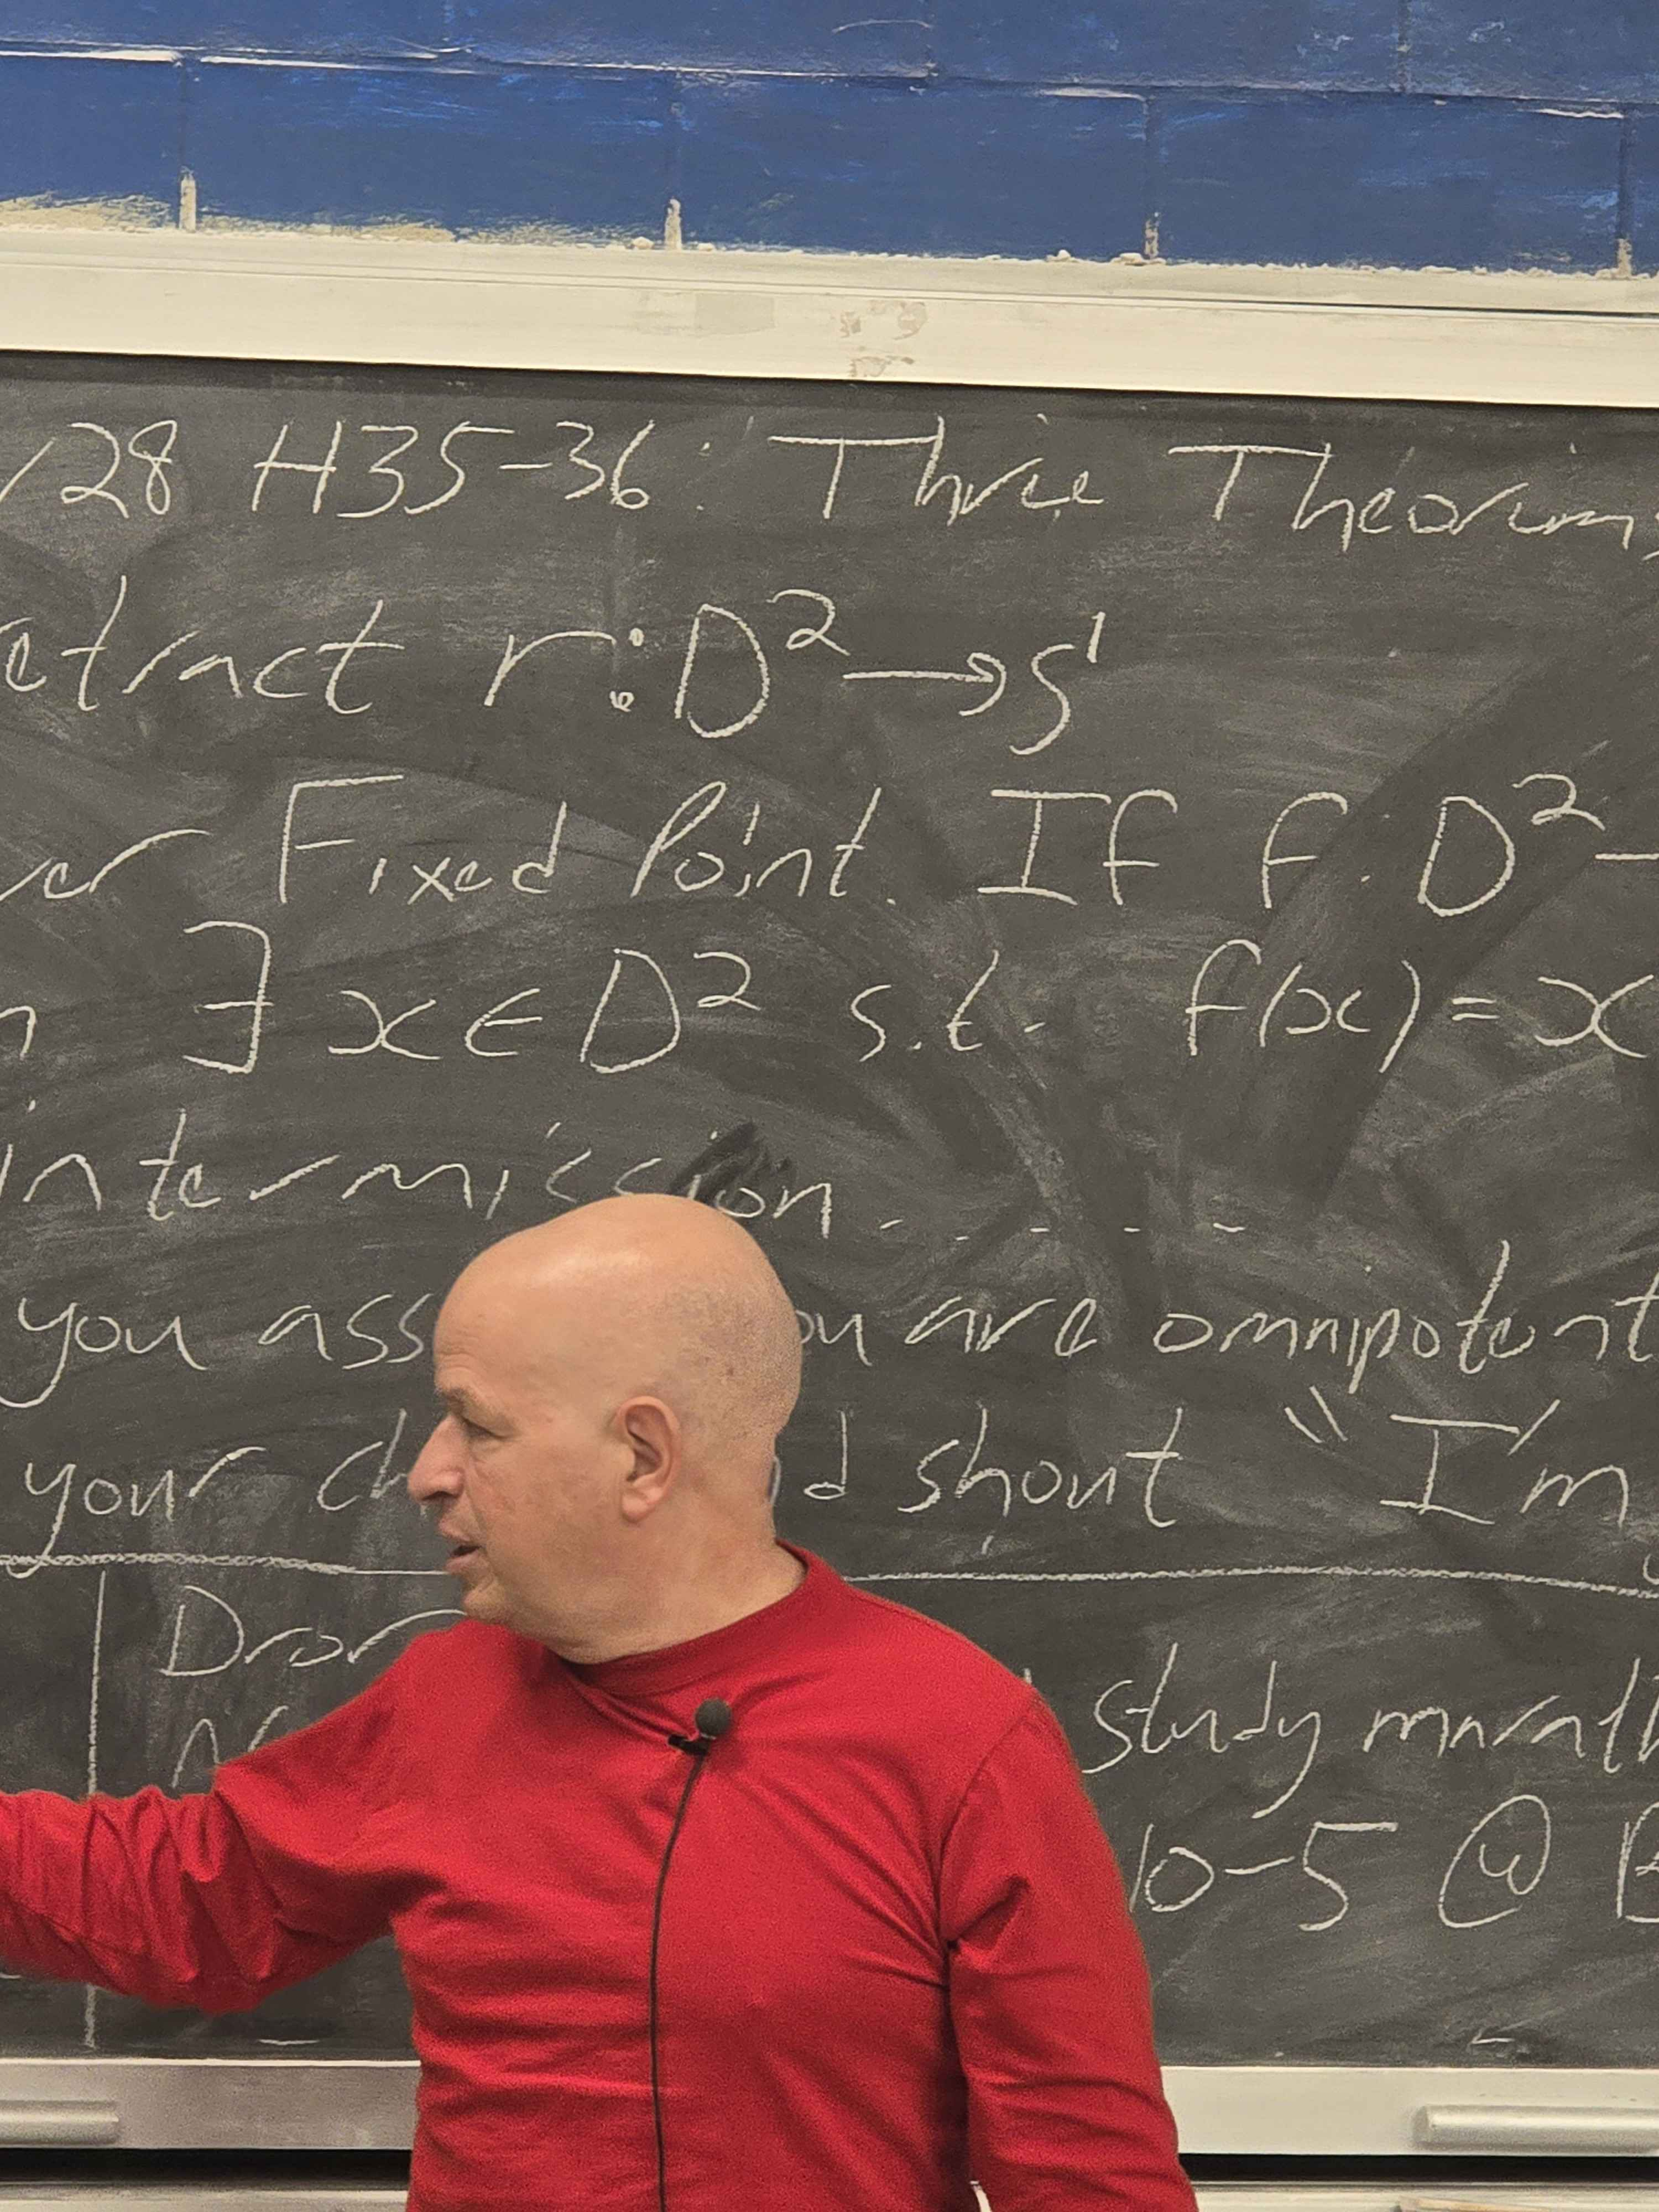
\includegraphics[scale=0.1]{MAT327 Notes/Dror Shirts/dror day 24 shirt.jpg}
\end{figure}

\noindent \textbf{Office hours information!}
\begin{itemize}
    \item Brinda will host office hours on Friday on Dec. 13, from 10am to 1pm in the grad lounge.
    \item Dror will not host office hours on Dec. 3, but will host them on Dec. 10, and will be available for a ``study marathon'' on Sunday, Dec. 15, from 10am to 5pm on Bahen's 6th Floor. He will roam around looking for topology students.
\end{itemize}

We will prove three major theorems today.
\begin{enumerate}[label=(\roman*)]
    \item There does not exist a retract $r : D^2 \to S^1$.
    \item (Brouwer Fixed Point Theorem) If $f : D^2 \to D^2$ is continuous, then there exists $x \in D^2$ such that $f(x) = x$.
    \item If you assume you are omnipotent, you get the pound on your chest and shout ``I'm great!''
\end{enumerate}
Recall that we have the following tools for today's lecture:
\[ \pi_1(\RR) = 0; \hspace{0.2in} \pi_1(S^1) = \ZZ, \]
and that $\pi_1$ is a functor, i.e.
\[
    \begin{tikzcd}
        X \arrow[r, rightsquigarrow, "\pi_1"] \arrow[loop left, "\id_X"] \arrow[d, "F"'] & \pi_1(X) \arrow[d, "\pi_1 f = f_\ast"] \\
        Y \arrow[r, rightsquigarrow, "\pi_1"'] \arrow[loop left, "\id_Y"] & \pi_2(Y)
    \end{tikzcd}
\]
We now prove the aforementioned theorems.
\begin{simplethm}[No Retraction]
    There does not exist a retract $r : D^2 \to S^1$.
\end{simplethm}
\noindent Suppose $r$ exists. Then we have the following diagram,
\[
    \begin{tikzcd}
        S^1 \arrow[r, hookrightarrow, "\iota"] \arrow[rd, "I"']& D^2 \arrow[d, "r"{name=L}] & \ZZ \arrow[r, "\pi_1 \iota"] \arrow[rd, "I"'{name=R}] & \{e\} \arrow[d, "\pi_1 r"] \\
        & S^1 & & \ZZ \arrow[from=L, to=R, start anchor = {[xshift=1ex]}, end anchor = {[xshift=-2ex, yshift=1.3ex]}, rightsquigarrow, "\pi_1"]
    \end{tikzcd}
\]
More generally, there does not exist a retraction $D^n \to S^{n-1}$ for $n > 2$, but this result will not be tested on the final. The proof is identical as the above, except we need a different functor.

\begin{simplethm}[Brouwer Fixed Point]
    If $f : D^2 \to D^2$ is continuous, then there exists $x \in D^2$ such that $f(x) = x$.
\end{simplethm}
\noindent By contradiction, assume $f : D^2 \to D^2$ is continuous and fro all $x$, $f(x) \neq x$. Let $r(x)$ be the point where the straight ray from $f(x)$ to $x$ is continuous, and hits the circle. Then $r(x)$ is continuous; if $x \in S^1$, then $r(x) = x$. So $r : D^2 \to S^1$ is a retract, but retracts don't exist. \qed

\begin{simplethm}[Formality of Limit]
    Assuming the axiom of choice, then let $\mathrm{Lim}$ be a function be from bounded sequences to $\RR$ such that
    \begin{enumerate}[label=(\roman*)]
        \item $\mathrm{Lim}$ is linear, i.e. $\mathrm{Lim}(a_n + b_n) = \mathrm{Lim} \, a_n + \mathrm{Lim} \, b_n$, and $\mathrm{Lim} \, (ca_n) = c \mathrm{Lim} \, a_n$, 
        \item $\mathrm{Lim} (a_n b_n) = (\mathrm{Lim} \, a_n)(\mathrm{Lim} \, b_n)$
        \item $\mathrm{Lim} \, a \in \bigcap_n \overline{\{a_k \mid k \geq n\}}$. If $a$ is convergent, then $\mathrm{Lim} \, a = \lim a$.
    \end{enumerate}
\end{simplethm}